\section{Information stealing vs consumer attack tree}
This section describes the attack tree for people who want to steal information from the consumer.
Some of the possible actors that want to obtain information from the consumer:
\begin{itemize}
\item Google, for better individual search
\item Commercial company, to better aim advertisements and commercials directly to the consumer
\item Appliance company, same as above and to know something about their market share and their competition
\item Intelligence agency, for surveillance
\end{itemize}

\begin{figure}
  \begin{center}
    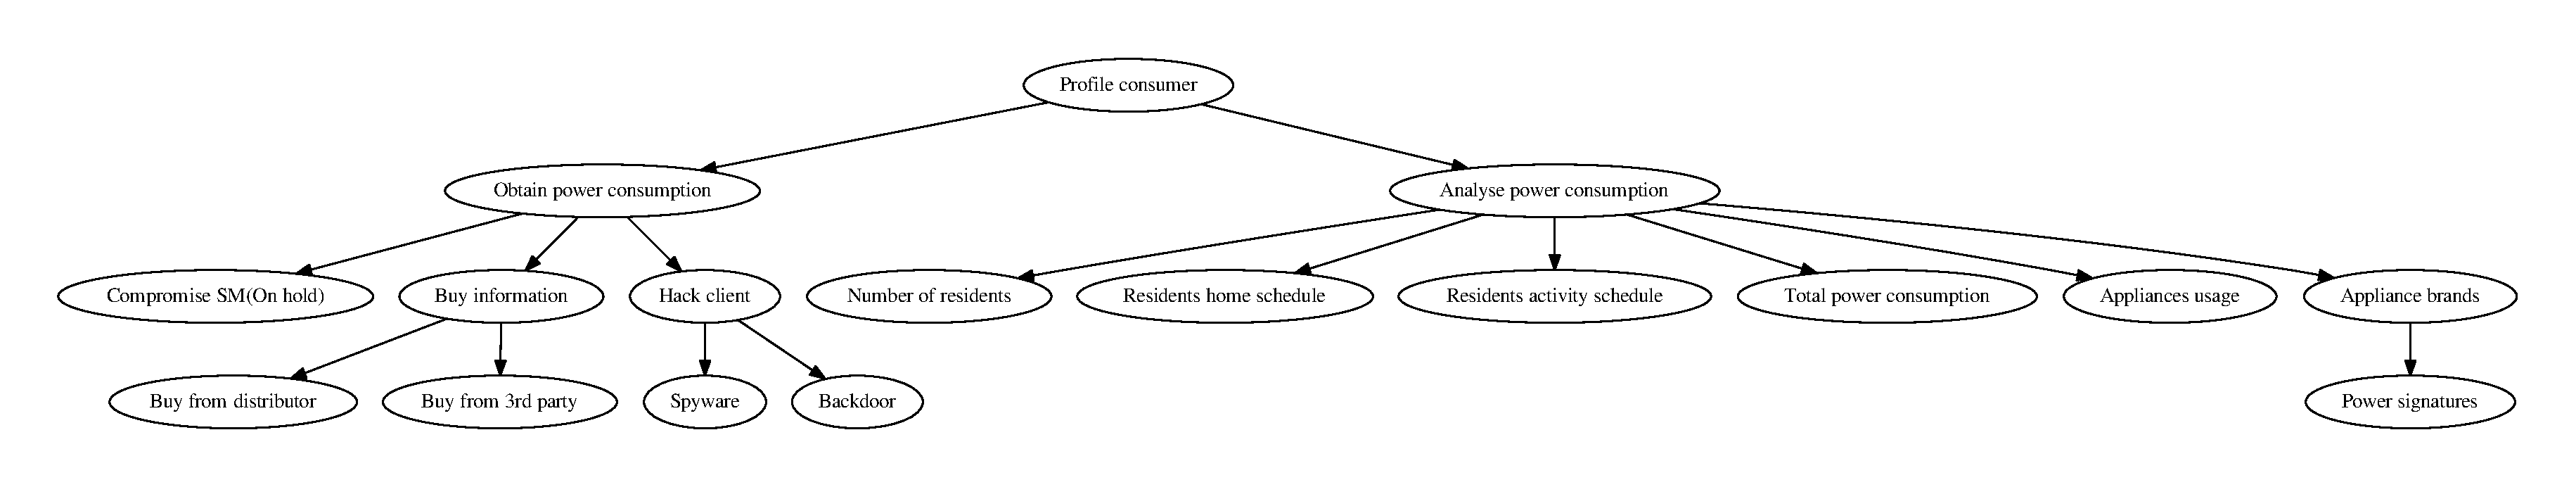
\includegraphics[angle=90, height=\textheight]{graphviz/information_stealing_vs_consumer_tree.pdf}
  \end{center}
  \caption{Information stealing from the consumer.}
  \label{information_stealing_tree}
\end{figure}

The attack tree can be seen on \cref{information_stealing_tree}.

\paragraph{Compromise smart meter}
Find vulnerabilities or backdoors to compromise the smart meter so it is possible to obtain information.
\bruno{more stuff here..}

\paragraph{Possibilities}
After gaining access to the smart meter and the consumption data there are many things that can be revealed about the household and the consumers activities and appliances.
See \cref{smart_meter_privacy} to see an example of how the consumption data could be used to reveal this information.
